\documentclass{article}
\usepackage{geometry}
\usepackage{graphicx}
\usepackage{amsmath}
\usepackage{algorithm}
\usepackage{algpseudocode}
\usepackage{dsfont}
\usepackage{amssymb}
\usepackage{multicol}

\geometry{
a4paper,
right=10mm,
left=10mm,
top=10mm,
bottom=10mm,	
}

\begin{document}

\pagenumbering{gobble}

\begin{center}
\textbf{\Large Assignment 1 : CS785} \\
\textit{\large Jayant Agrawal}         14282
\end{center}

\section{Car Accident}
\section{Watergate scandal}
\textbf{(a)} \\
If the decision is \emph{6-2}, then it is better for the president to defy rather than comply, arguing that the split decision can not bind him. But, in this case the Court would not have enough evidence to prosecute him, hence they are worse off. If the decision is \emph{8-0}, then the president has to comply because if he defies, then it would probably lead to his impeachment. Thus, the payoff for comply is better than defy. Also, if he complies, then the Court would have enough evidence to prosecute, thus their payoff is better in this case.\\
\textbf{(b)}
\begin{figure}[h!]
\centering
\begin{multicols}{3}
\label{2_gt1}
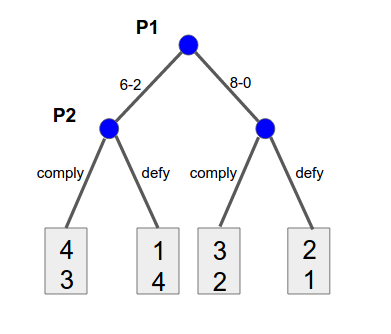
\includegraphics[width=1\columnwidth]{2_gt1.png}
\caption{Game Tree}


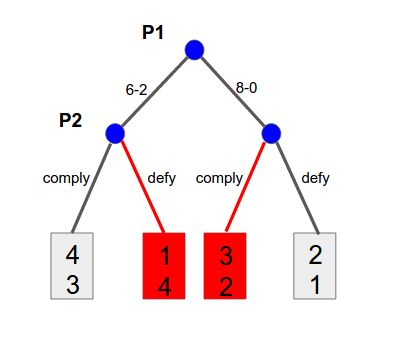
\includegraphics[width=1\columnwidth]{2_gt2.png}
\caption{Backward Induction: Player 2}
\label{2_gt2}


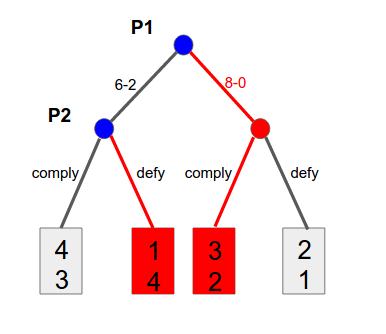
\includegraphics[width=1\columnwidth]{2_gt3.png}
\caption{Backward Induction: Player 1}
\label{2_gt3}
\end{multicols}
\end{figure}

By Backward Induction, \emph{Player 2 argues} that if the decision is \emph{6-2}, then it is better to \emph{defy}, since $4$ is better than $3$. If the decision, is \emph{8-0}, then it is better to \emph{comply}, since $2$ is better than $1$. This is illustrated in Figure \ref{2_gt2}. Now, \emph{Player 1 argues} that if the decision is \emph{6-2}, then Player 2 will \emph{defy} and the payoff is $1$. But, if the decision is \emph{8-0}, then Player 2 will comply and the payoff is $3$. Therefore, \emph{8-0} is better. \\ \\
Thus, the predicted outcome is \emph{\{ 8-0, comply \}}. \\ \\
\textbf{(c)} \\
Nixon could have a better outcome if he had successfully influenced the 2 judges to give the decision in his favour and then defy the judgement, arguing that a split decision can not bind the President. His payoff would then be 4 instead of 2.\\ \\
\textbf{(d)} \\
The Supreme Court gave an \emph{8-0} decision and the President had to comply and hand-over the tapes(he also resigned after 16 days).
\section{Campus Shops}
\textbf{(a)} Let the price chosen by $S1$ be $p_1$, then if $S2$ choses $p_2$, the revenue generated by $S1$ and $S2$ is: 
$$\pi_{1} = p_1 \times (10-2p_1-p_2)$$
$$\pi_{2} = p_2 \times (10-p_1-2p_2)$$
Now, given $p_1$, $S2$ will choose $p_2$ such that $\pi_2$ is maximum, or:
$$\frac{\partial \pi_2}{\partial p_2}= 0$$
$$ 10 - p_1 -4p_2  = 0$$
$$p_2 = \frac{10-p_1}{4}$$
Now, since $S1$ knows the above strategy of $S2$, it will choose $p_1$, such that $\pi_1$ is maximum, given the above value of $p_2$:
$$\frac{\partial \pi_1}{\partial p_1}= 0$$
$$\frac{\partial}{\partial p_1}\Big(10p_1 - 2p_1^2 -p_1(\frac{10-p_1}{4})\Big)= 0$$
$$10 - 4p_1 - 10/4 + p_1/2 = 0$$
$$p_1 = 15/7 \sim 2.14$$
Therefore $p_2 = 55/28 \sim 1.96$. Thus, revenues are $\pi_1 = 8.03$ and $\pi_2 = 7.72$
\section{Tax Rate}
\section{Wireless Spectrum Block}
Suppose the government(Player 1) announces a tax rate $r$, and the citizens(Player 2) put effort $e$, then the respective payoff are:
$$ \pi_1 = r \times (4e - 4re - e^2)$$
$$ \pi_2 = (1-r) \times (4e - 4re - e^2)$$
Given $r$, citizens would put effort $e$, such that their payoff($\pi_2$) is maximum:
$$\frac{\partial \pi_2}{\partial e}= 0$$
$$ 4(1-r)- 4r(1-r) - 2(1-r)e = 0$$
$$e = 2(1- r), r \neq 1$$
Since the government would know the above strategy of the citizens, it would choose r such that their payoff ($\pi_1$) is maximum, given the above the value of e:
$$\frac{\partial \pi_1}{\partial r}= 0$$
$$\frac{\partial}{\partial r}\Big(r \times (8(1-r) - 8r(1-r) - 4(1-r)^2)\Big)= 0,r \neq 1$$
$$\frac{\partial}{\partial r}\Big(4r - 8r^2+4r^3\Big)= 0,r \neq 1$$
$$1 - 4r + 3r^2 = 0,r \neq 1$$
$$r = 1/3$$
Thus, the government would choose $r=1/3$ to maxmize it's payoff.

\section{Demonetised Note Auction}
\end{document}


